
\documentclass{article}
\usepackage{polyglossia}
\setdefaultlanguage{slovak}
\usepackage{graphicx}
\usepackage{hyperref}
\usepackage{gensymb}
\usepackage[dvipsnames]{xcolor}
\hypersetup{
	colorlinks=true,
	linkcolor=blue,
	urlcolor=red,
	filecolor=magenta
}
\urlstyle{same}
\title{Národný park Maasai Mara}
\author{Adam Jenča}
\begin{document}
\definecolor{sedocierna}{RGB}{50,50,50}
\pagecolor{white}
\color{sedocierna}
\maketitle
{{\tableofcontents{}}}
\newpage
\section{Úvod}
Park \textbf{Maasai Mara} je národný park na juhozápade Kene. Susedí z národným parkom Serengeti spolu s ním a inými časťami Kene a Tanzánie je súčaťou ekosystému Mara--Serengeti, v ktorom je mnoho druhov endemitmi(napríklad Perlavec masajský) Prvá časť jeho mena je názov miestneho domorodého kmeňa Masajov. Druhá časť pochádza z ich jazyka a značí fľakatý podľa nízkych stromov a krov, ktoré sa v jeho juhozápadnej časti vyskytujú dosť často. Z rovnakého slova pochádza aj názov rieky Mara, ktorá cez park preteká a je jeho hlavnou zásobiteľkou.

\begin{figure}[h]
\centering
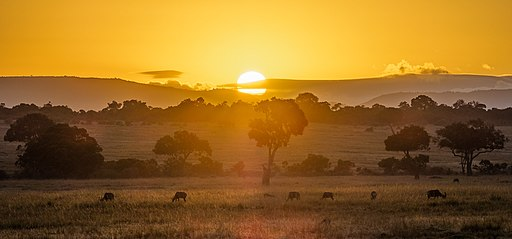
\includegraphics[scale=0.65]{mara-skvrnity.jpg} \caption{Pre toto sa volá park Masai Mara ,,škvrnitý''}
\end{figure}

\noindent
 \hyperref[sec:gmwildebe]{Migrácia pakoní} cez park patrí medzi Desať divov sveta a Sedem divov Afriky.
\vskip 5mm
%

\begin{figure}[h]
\centering
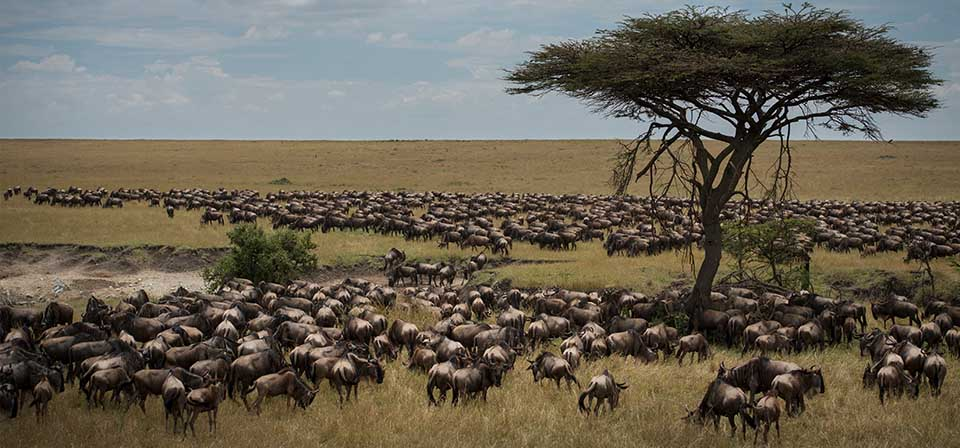
\includegraphics[scale=0.35]{migracia-velka.jpg} \caption{Migrujúce pakone}
\end{figure}


%\hrule
\section{História}
Prvá rezervácia na území parku vznikla v roku 1948 a mala nejasné hranice, ktoré boli oveľa kratšie.
Štatút národnej rezervácie jej bol udelený v roku 1974 a od roku 1984 má dnešné hranice.

\section{Geografia}

\begin{figure}[h]
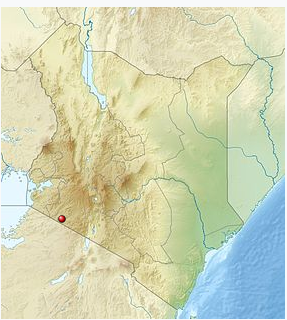
\includegraphics[scale=0.3]{location.png}\caption{Poloha parku Maasai Mara}
\end{figure} 
\medskip

\noindent
Park dosahuje veľkosť takmer 1510km$^2$. Terén je otvorená trávnatá plocha s akáciovými lesmi, lužnými lesmi a húštinami. Jeho hranice sú park Seregneti na juh, 
zráz Ololoo (súčasť Východoafrickej priekopovej prepadliny) na západ
a masajské pastviny na sever, západ a východ.

\noindent
Má stepnú klímu, takže v nej sú dve obdobia dažďov: jedno trvá šesť týždňov a je v apríli až v máji ; druhé trvá kratšie a je v novembri až v decembri.
Teplota je 12--30 \degree C
\noindent 
 
\newpage
\section{Flóra a fauna}
\subsection{Fauna}
Veľmi dôležitou súčasťou fauny celej Afriky je tzv. Veľká Päťka z ktorej všetky druhy žijú aj na území NP Maasai Mara:
\begin{flushright}
\begin{itemize}
\item Slon africký $($\texttt{\textit{Loxodonta Africana}}$)$ 
\includegraphics[scale=0.09]{VU.png}{\color{Dandelion} \textbf{Zraniteľný}}
\begin{figure}[h]
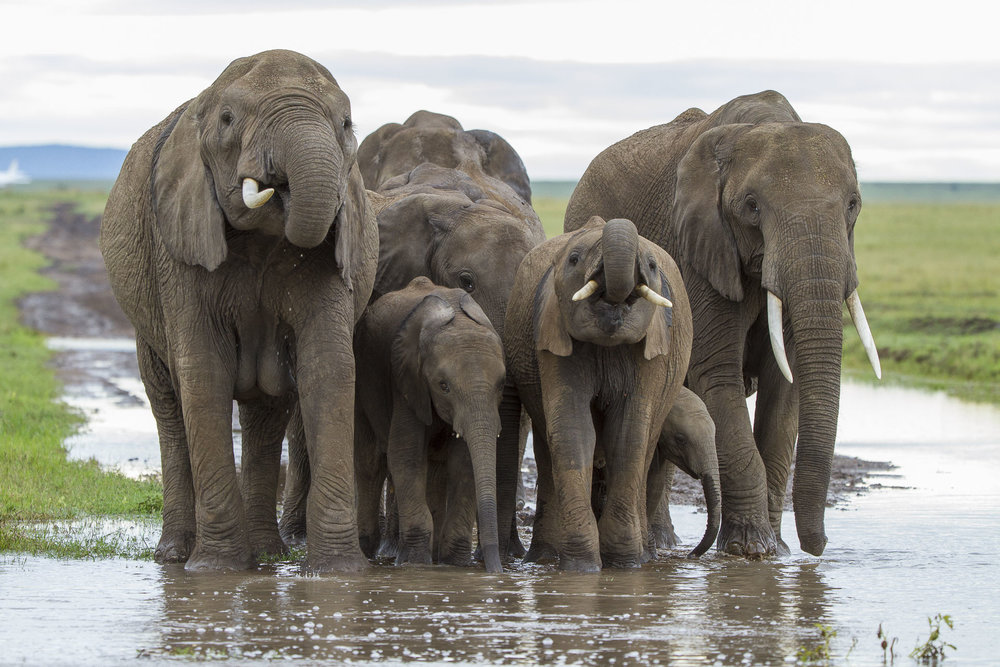
\includegraphics[scale=0.8]{Slony-masai.jpg}

\end{figure}



\item Byvol africký $($\texttt{\textit{Syncerus Caffer}}$)$ 
\includegraphics[scale=0.015]{LC.png}{\color{ForestGreen} \textbf{Najmenej ohrozený}}

\begin{figure}[h]

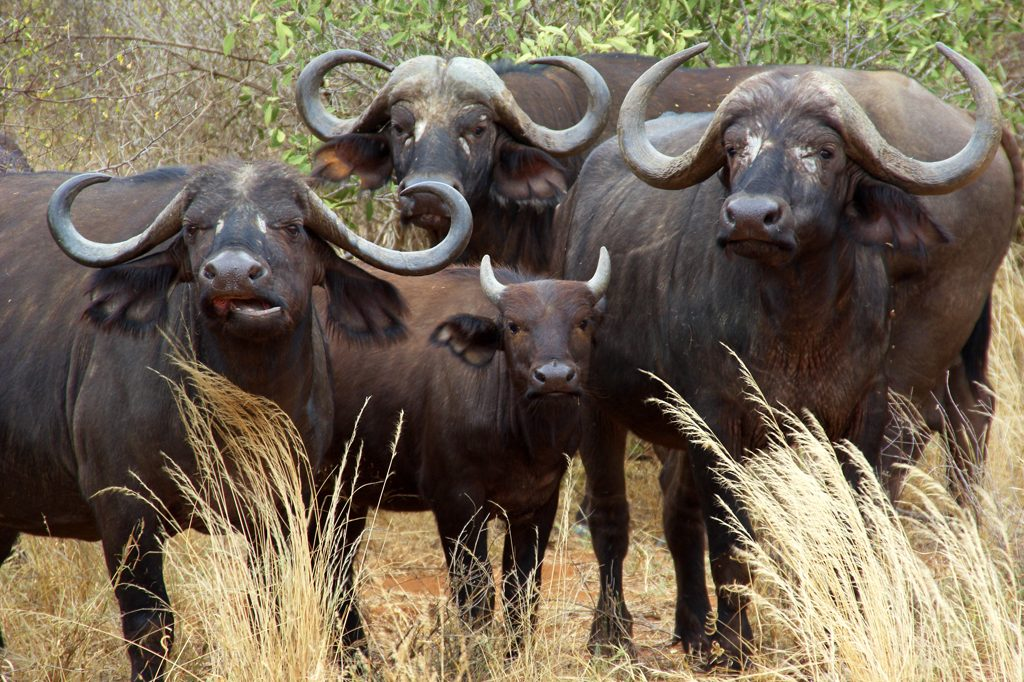
\includegraphics[scale=0.2]{byvoly-masai.jpg}
\end{figure}

\newpage
\item Nosorožec tuponosý južný(\texttt{\textit{Ceratotherium simum}}$)$
\includegraphics[scale=0.015]{NT.png}{\color{ForestGreen} \textbf{Blízko ohrozenia}}
\vskip 0.653in
\begin{figure}[h]

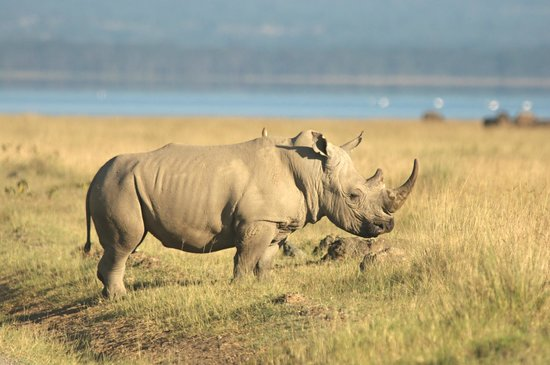
\includegraphics[scale=0.005]{nosoroh-masai.jpg}
\end{figure}
\item Lev púšťový $($\texttt{\textit{Panthera leo}}$)$
\includegraphics[scale=0.09]{VU.png}{\color{Dandelion}\textbf{Zraniteľný}}

\begin{figure}[h]

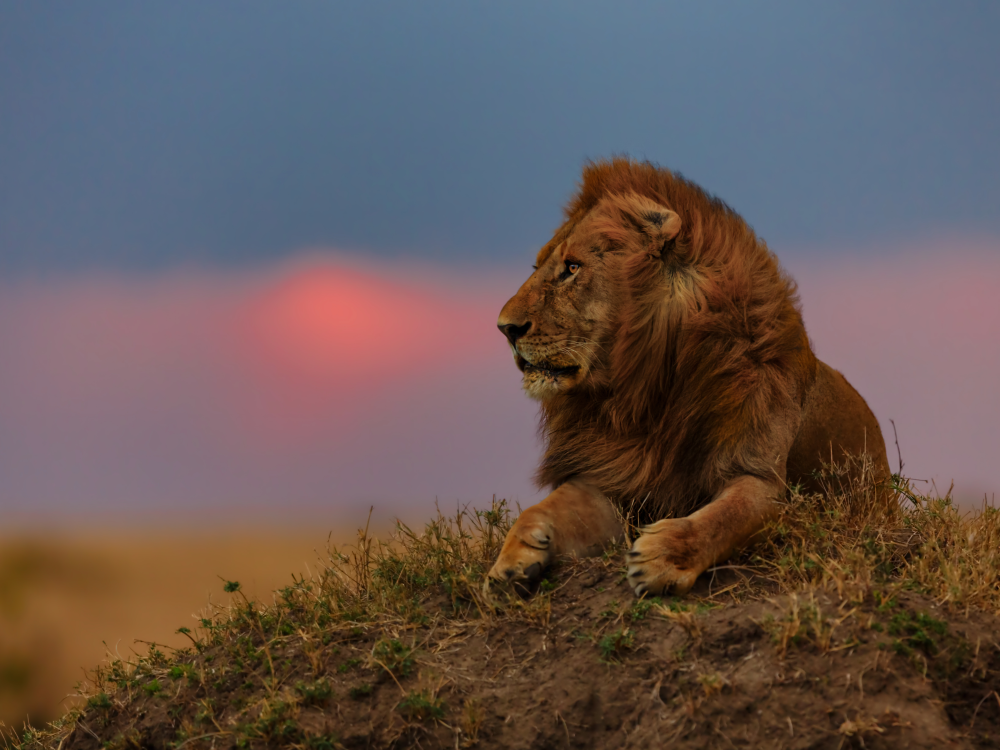
\includegraphics[scale=0.4]{lev-masai.png}
\end{figure}
\newpage
\item Leopard škvrnitý $($\texttt{\textit{Panthera pardus}}$)$
\includegraphics[scale=0.09]{VU.png}{\color{Dandelion}\textbf{Zraniteľný}}
\begin{figure}[h]
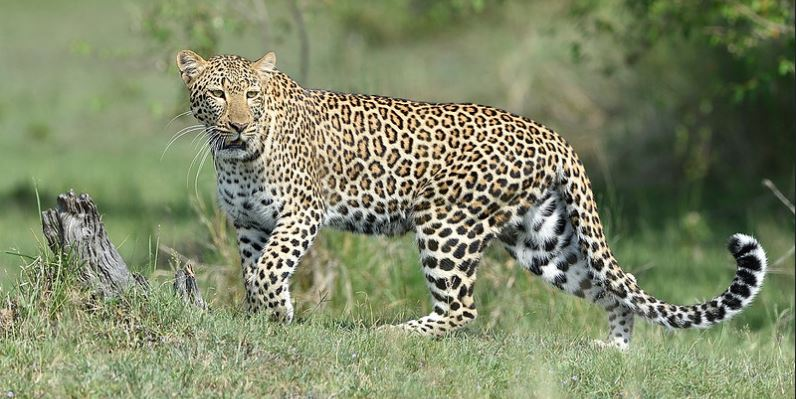
\includegraphics[scale=0.4]{leopard-masai.jpg}
\end{figure}
\end{itemize}
\end{flushright}
Pakôň pásavý  $($\texttt{\textit{Connochates taurinus}}$)$
\includegraphics[scale=0.015]{LC.png}{\color{ForestGreen} \textbf{Najmenej ohrozený}}\\

Pakôň je zaujímavý tým, že sa zhromažďuje do miliónových skupín a migruje po Východnej Afrike. Je nezvyčajné, aby sa zvieratá spájali do takých obrovských skupín, preto je tento jav zaradený do 7 divov Afriky. \hyperref[sec:gmwildebe]{Viac}\\
\vskip 2mm 
\begin{figure}[h]
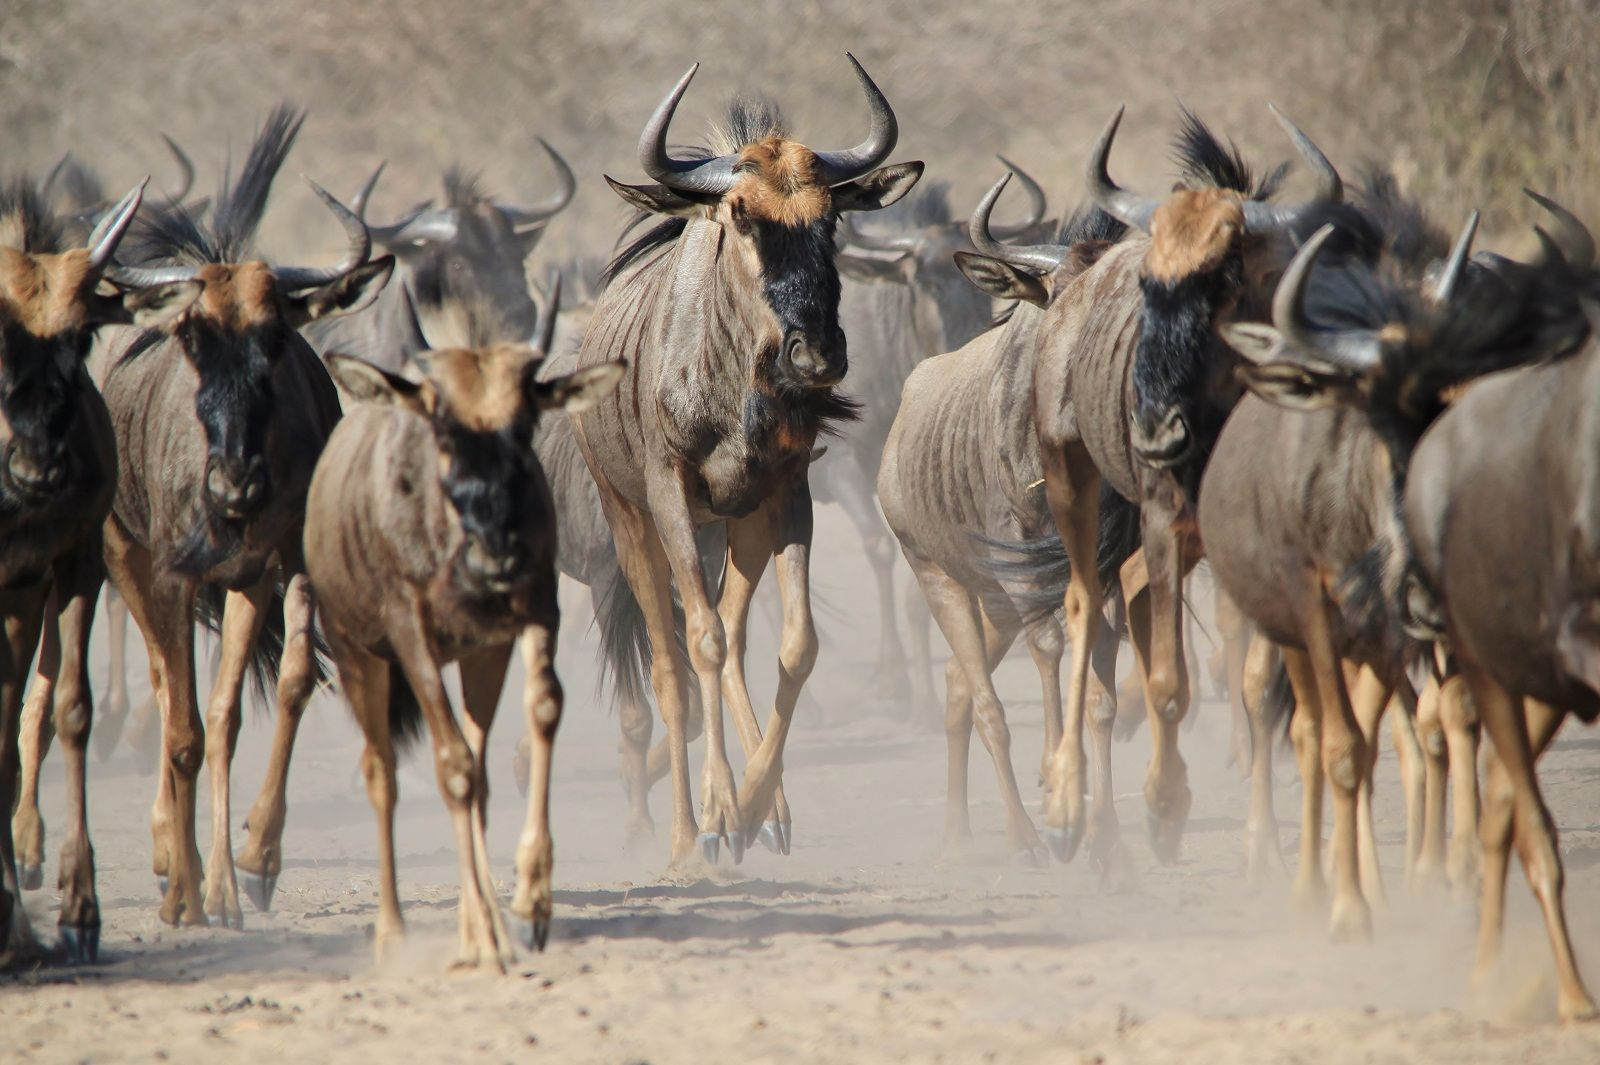
\includegraphics[scale=0.6]{pakone-masai.jpg}
\end{figure}
\newpage
\subsection{Flóra}
Flóra NP Maasai Mara sa skladá hlavne z tráv a suchomilných stromov a krov, ale časti pozdĺž riek Mara a Talek sa vyznačujú stromami a močiarnymi rastlinami typickými pre lužné lesy.

\begin{figure}[h]
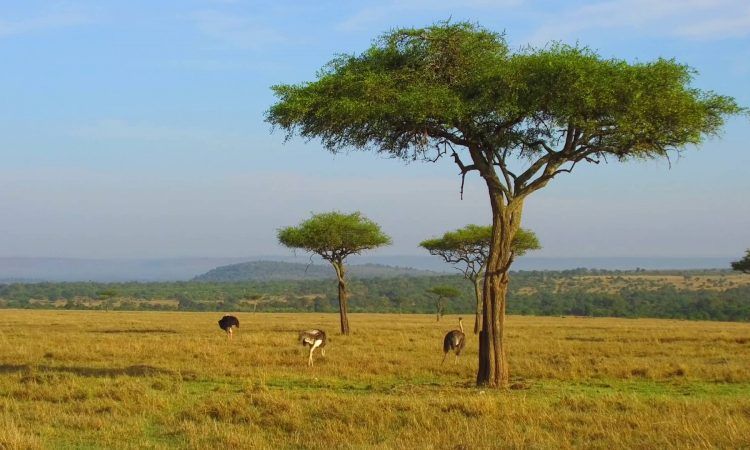
\includegraphics[scale=0.3]{datlovnik.jpg}
\caption{Typická ,,suchá''flóra parku Maasai Mara}
\end{figure}
\begin{figure}[h]
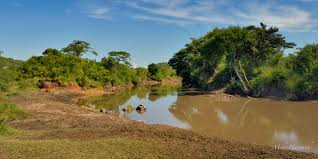
\includegraphics[scale=1.0]{riverine.jpeg}
\caption{Lužné lesy v parku Maasai Mara}
\end{figure}
\newpage
\subsection{Veľká Migrácia}
\label{sec:gmwildebe}
\begin{figure}[t]
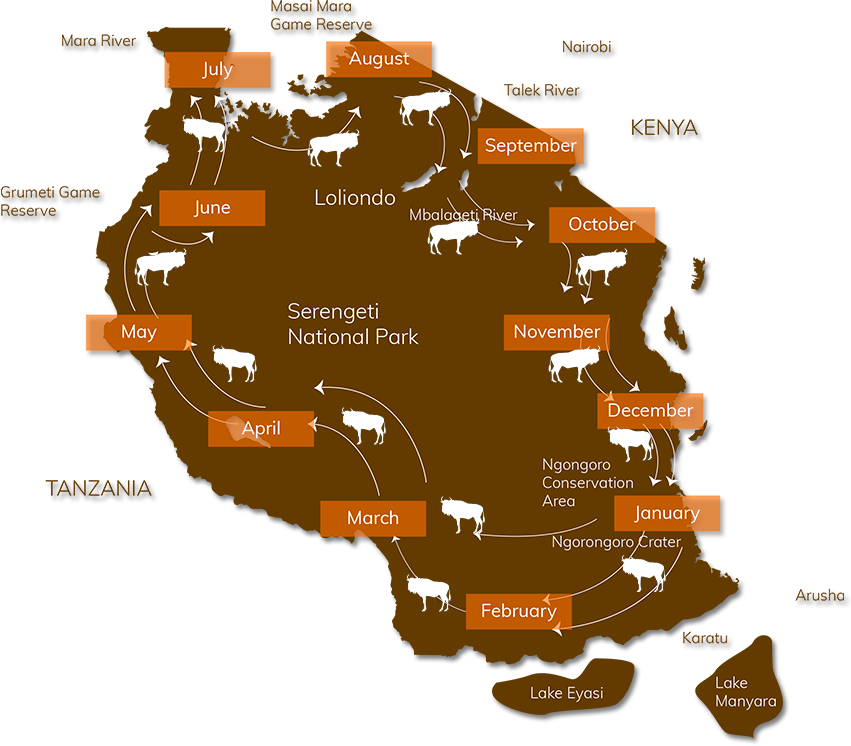
\includegraphics[scale=0.2]{map.png}
\caption{Mapa Veľkej migrácie}
\end{figure}
Veľká Migrácia je migrácia pakoní, ktorú v parku môžete vidieť približne od júna do októbra.
Pakone migrujú v cykle:
\begin{enumerate}
\item sever parku Serengeti
\item park Masai Mara, v ňom zostávajú počas zimy(park je južne od rovníka)
\item kráter Ngorngoro, Tanzánia:tu koncom januára porodia mladé
\item jazero Ndutu
\item sever parku Serengeti
\end{enumerate}
Masai Mara je najlepším miestom na sledovanie tohto javu, ktorý sa radí medzi 7 Divov Afriky a medzi 10 Divov sveta.
Hovorí sa, že scéna, pri ktorej pakone prechádzajú rieku Mara je jednoducho úchvatná.
\vskip 1cm
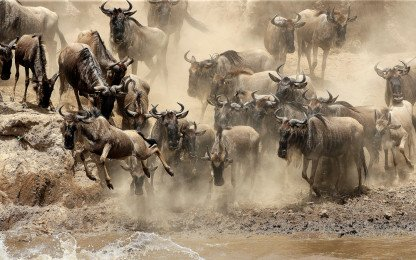
\includegraphics[width=0.5\textwidth,natwidth=200,natheight=200]{pakone-mara.jpg}\\
\center{\textbf{Obr.6} Pakone prechádzajúce cez rieku Mara}
	\subsection{Vtáctvo}
\label{subsec:brdng}
\href{https://raw.githubusercontent.com/jenca-adam/masai-mara-birding/master/vtactvo.txt}{\textbf{Zoznam vtákov v parku Masai Mara}}\\ 
Vtáctvo v parku Masai Mara si zaslúži osobitnú zmienku. V parku žije okolo 500 druhov vtákov, z toho 57 dravcov. 
Sťahovavé vtáky tu zostávajú od novembra do apríla.
Niektoré vtáky v parku :\\
\begin{itemize}
\item Drop najväcší $($\texttt{\textit{Ardeotis kori}}$)$
\includegraphics[scale=0.015]{NT.png}{\color{ForestGreen}\textbf{Blízko ohrozenia}}

\vskip 2.473927392948942843982cm
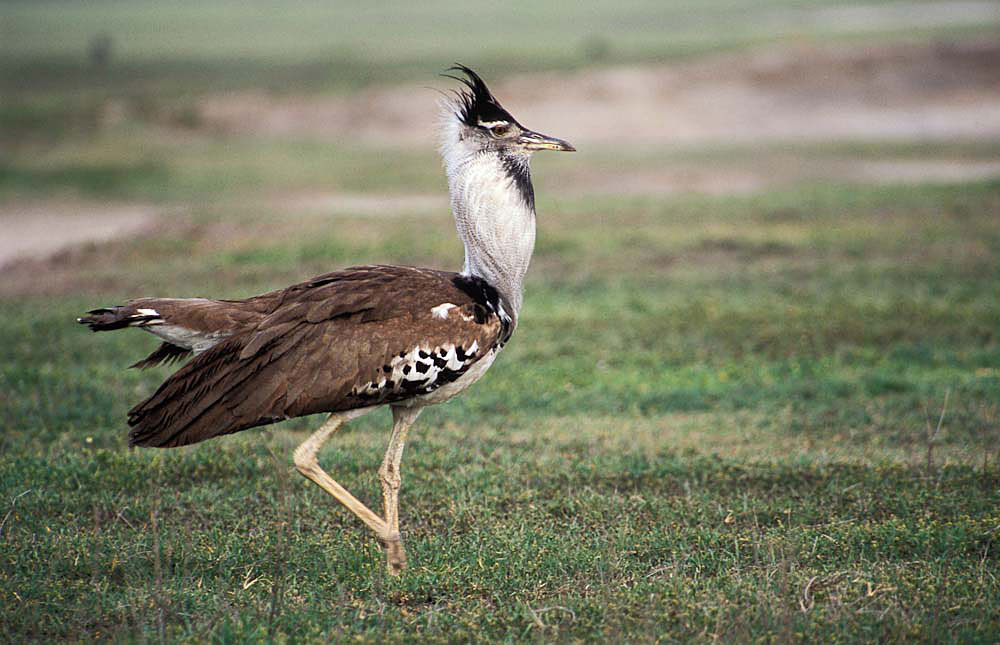
\includegraphics[width=0.09\textwidth,natwidth=200,natheight=200]{kori-masai.jpg}\\
\item Čaplička hnedobruchá $($\texttt{\textit{Ardeola rufiventris}}$)$
\includegraphics[scale=0.015]{LC.png}{\color{ForestGreen} \textbf{Najmenej ohrozený}}

\vskip 2.473927392948942843982cm

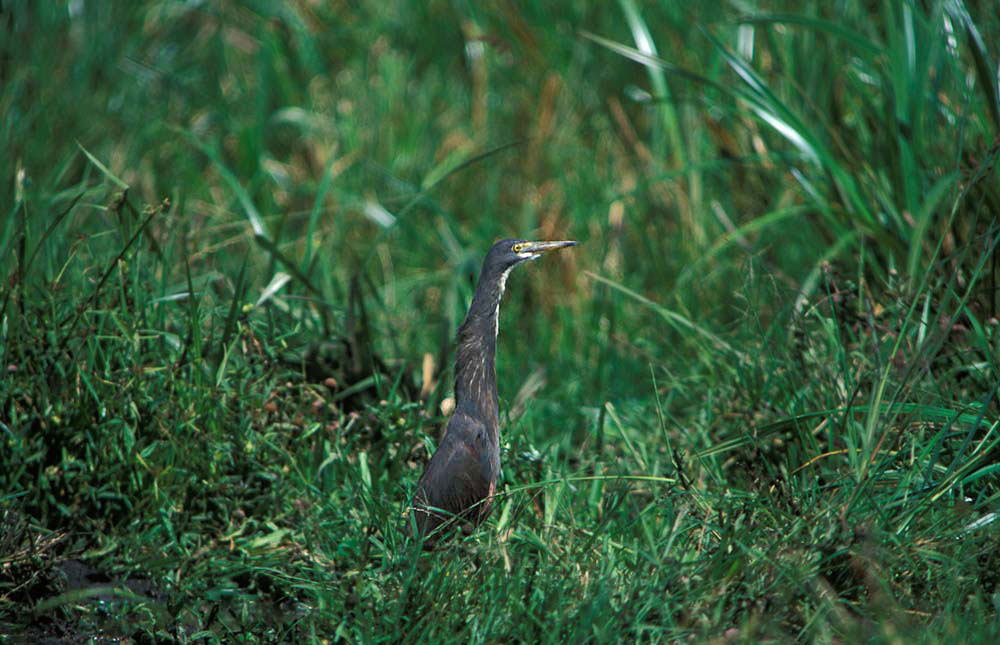
\includegraphics[width=0.09\textwidth,natwidth=200,natheight=200]{caplicka-masai.jpg}\\
\item Hadožrút nohatý$($\texttt{\textit{Sagittarius serpentarius}}$)$
\includegraphics[scale=0.09]{VU.png}{\color{Dandelion}\textbf{Zraniteľný}}

\vskip 2.473927392948942843982cm
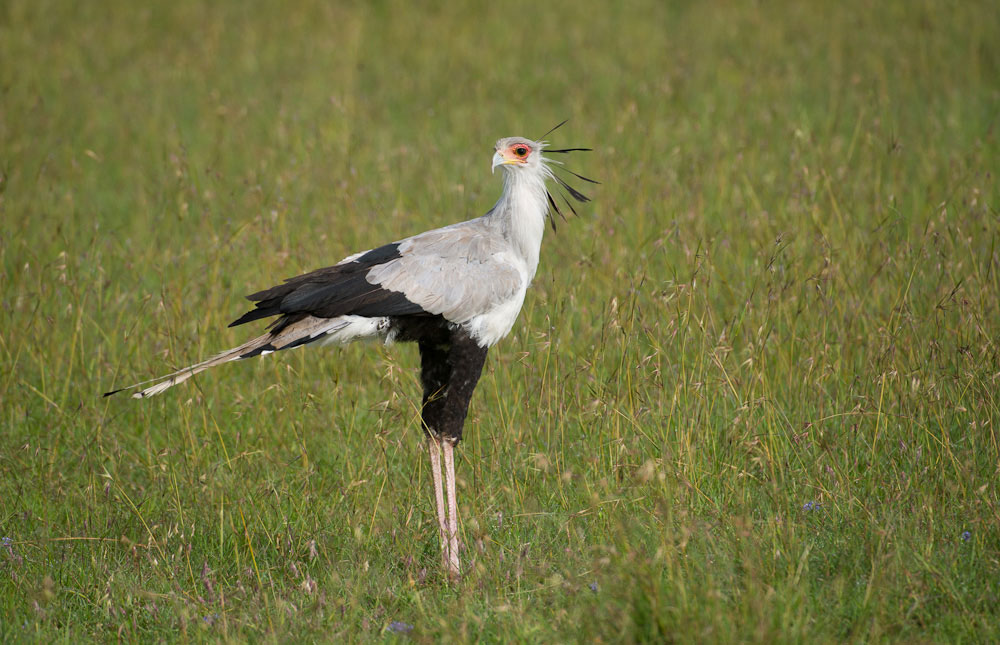
\includegraphics[width=0.09\textwidth,natwidth=200,natheight=200]{hadozrut-masai.jpg}\\
\item Perlavec masajský$($\texttt{\textit{Trachyphonus darnaudii usambiro}}$)$
\includegraphics[scale=0.015]{LC.png}{\color{ForestGreen} \textbf{Najmenej ohrozený}}

\textit{Endemit v ekosystéme Mara--Serengeti}
\vskip 2.473927392948942843982cm
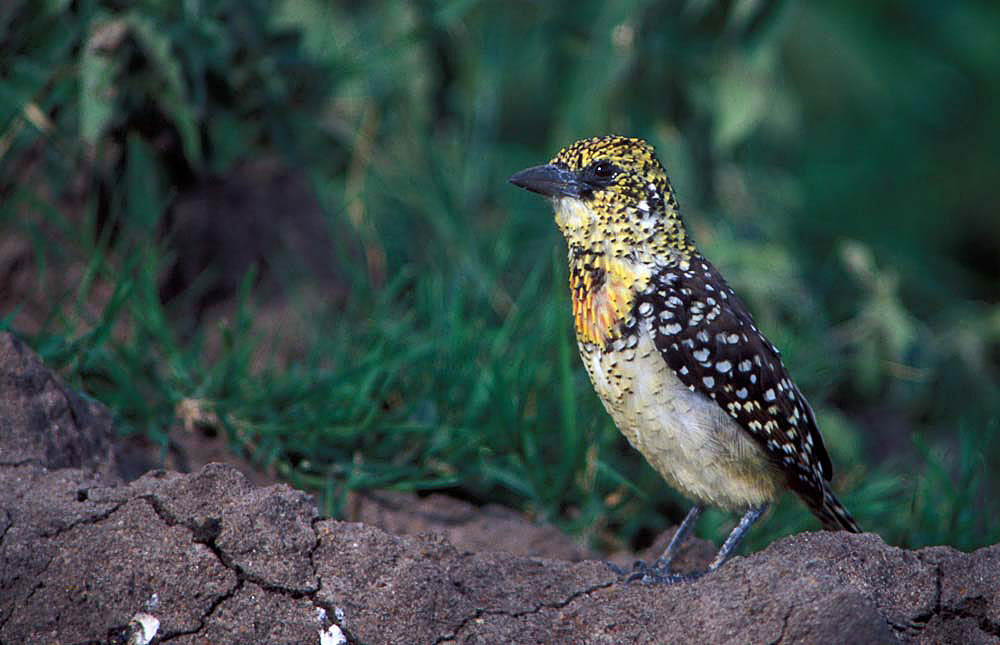
\includegraphics[width=0.09\textwidth,natwidth=200,natheight=200]{usambiro-masai.jpg}\\

\end{itemize}
\section{Zdroje}
\begin{itemize}

\item \url{https://www.safaribookings.com/masai-mara/wildlife}(Fauna)
\item \url{https://www.safaribookings.com/masai-mara/birding/}(Vtáctvo)
\item \url{https://en.wikipedia.org/wiki/Maasai_Mara}(Poloha,História)
\end{itemize}
 {\small \textit{Made using \LaTeX{}}}
\end{document}
